\documentclass[border=6pt]{standalone}
\usepackage{tikz}
\usetikzlibrary{arrows.meta,positioning,calc,fit,backgrounds}

\definecolor{ink}{HTML}{0F172A}
\definecolor{muted}{HTML}{64748B}
\definecolor{linegray}{HTML}{CBD5E1}
\definecolor{panel}{HTML}{F8FAFC}
\definecolor{sourcefill}{HTML}{ECFEFF}
\definecolor{sourcestroke}{HTML}{0891B2}
\definecolor{batteryfill}{HTML}{F0FDF4}
\definecolor{batterystroke}{HTML}{15803D}
\definecolor{fusefill}{HTML}{FEF2F2}
\definecolor{fusestroke}{HTML}{DC2626}
\definecolor{gearfill}{HTML}{EEF2FF}
\definecolor{gearstroke}{HTML}{4F46E5}
\definecolor{busfill}{HTML}{FEF9C3}
\definecolor{busstroke}{HTML}{A16207}
\definecolor{poswire}{HTML}{B91C1C}
\definecolor{negwire}{HTML}{334155}
\definecolor{acwire}{HTML}{0369A1}

\begin{document}
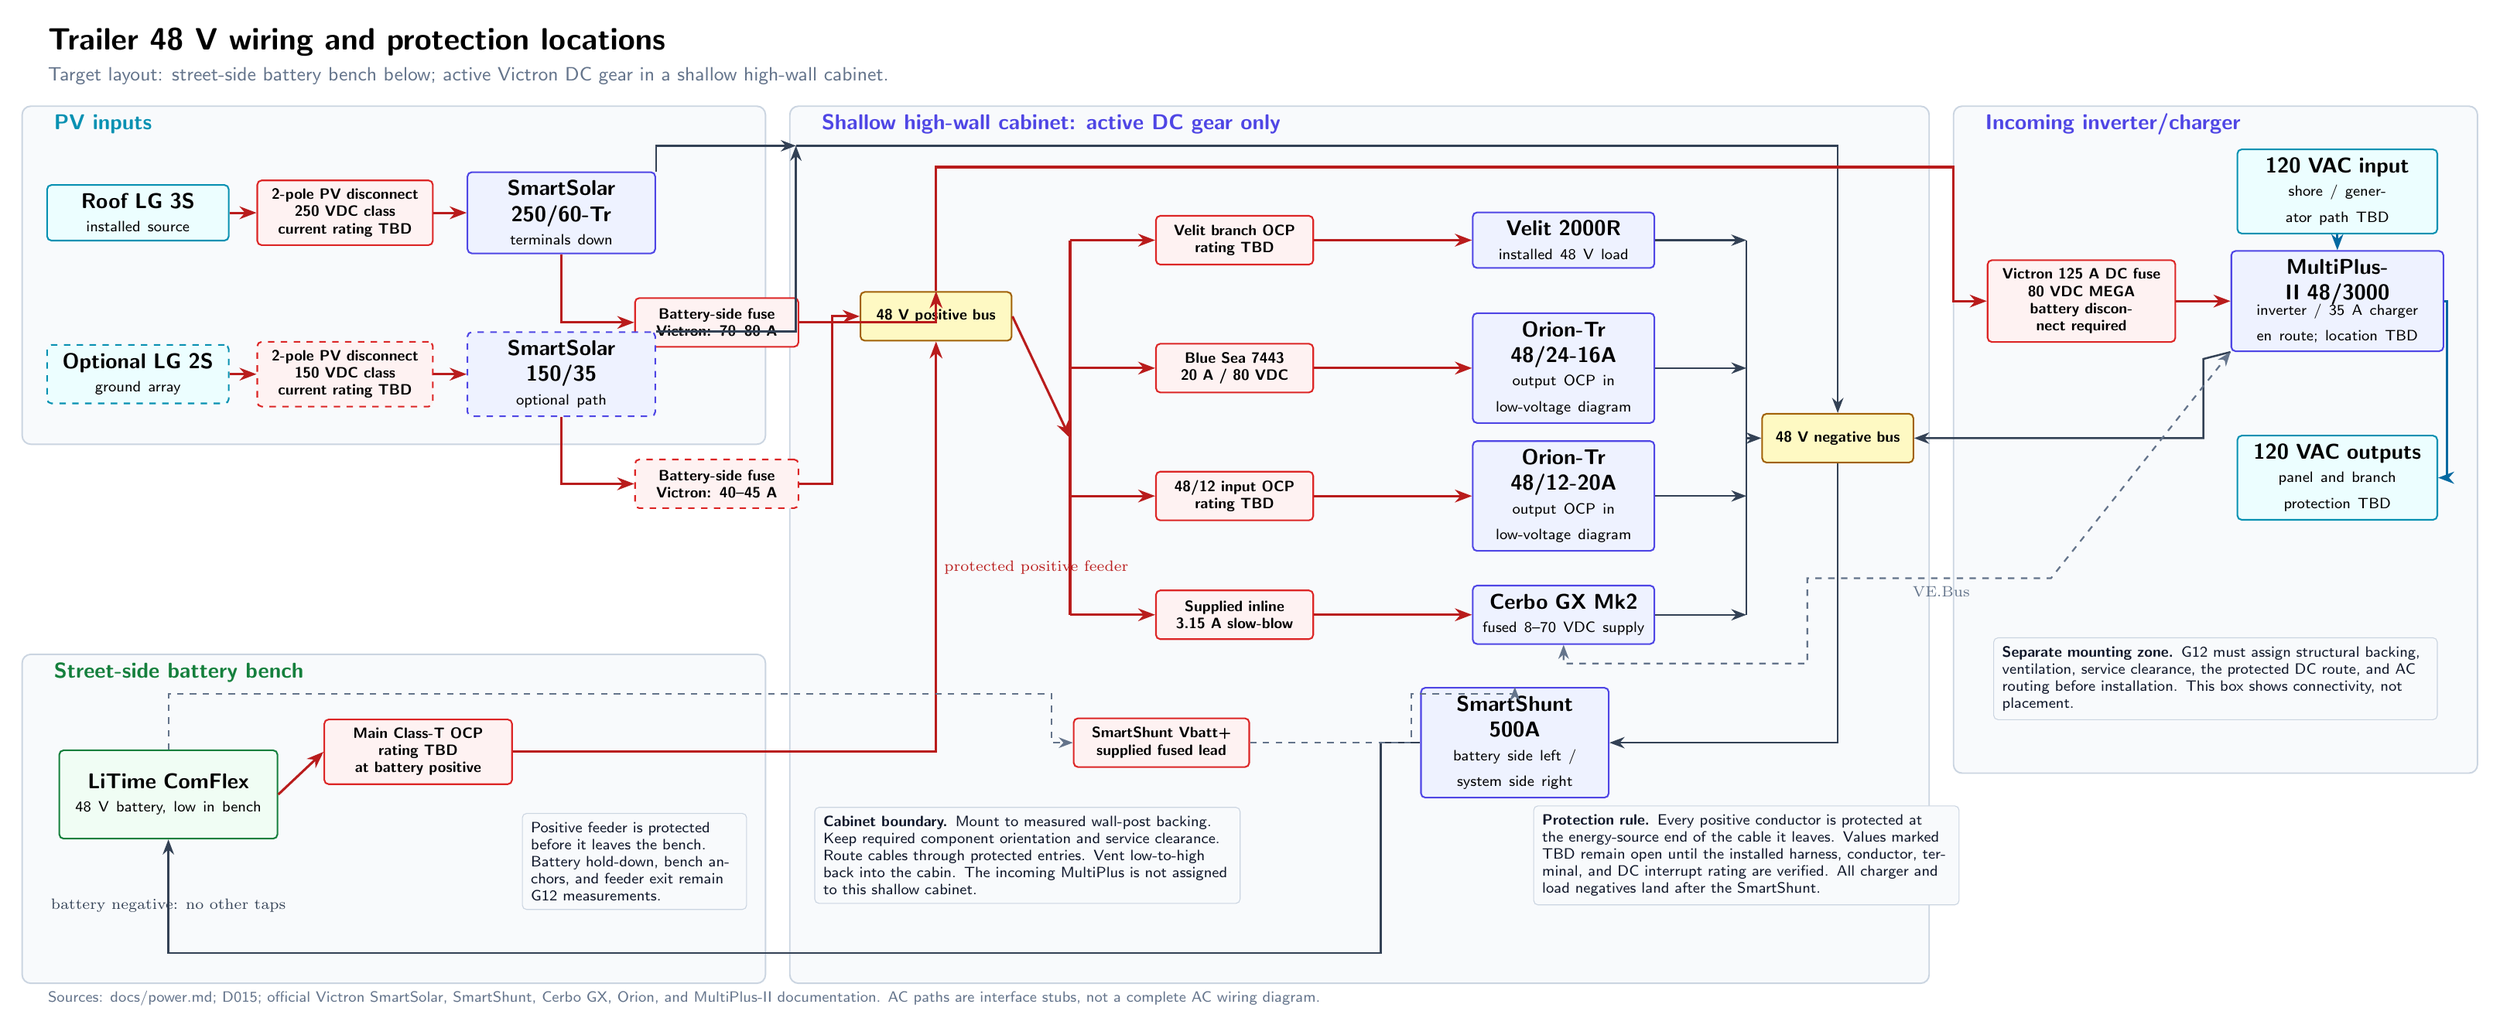
\begin{tikzpicture}[
  font=\sffamily,
  >=Stealth,
  block/.style={draw=ink, fill=white, rounded corners=2pt, line width=0.75pt,
    align=center, inner sep=4pt, minimum height=0.8cm},
  source/.style={block, fill=sourcefill, draw=sourcestroke},
  battery/.style={block, fill=batteryfill, draw=batterystroke},
  gear/.style={block, fill=gearfill, draw=gearstroke},
  fuse/.style={block, fill=fusefill, draw=fusestroke, font=\sffamily\scriptsize\bfseries},
  bus/.style={block, fill=busfill, draw=busstroke, font=\sffamily\scriptsize\bfseries},
  note/.style={draw=linegray, fill=panel, rounded corners=2pt, align=left,
    inner sep=4pt, font=\sffamily\scriptsize, text=ink},
  zone/.style={draw=linegray, fill=panel, rounded corners=4pt, line width=0.7pt},
  positive/.style={->, draw=poswire, line width=1.1pt},
  neg/.style={->, draw=negwire, line width=0.9pt},
  sense/.style={->, draw=muted, line width=0.8pt, dashed},
  ac/.style={->, draw=acwire, line width=1.0pt},
  control/.style={<->, draw=muted, line width=0.8pt, dashed}
]

\node[font=\sffamily\bfseries\Large, anchor=west] at (0,15.7)
  {Trailer 48 V wiring and protection locations};
\node[font=\sffamily\small, text=muted, anchor=west] at (0,15.15)
  {Target layout: street-side battery bench below; active Victron DC gear in a shallow high-wall cabinet.};

\begin{scope}[on background layer]
  \node[zone, fit={(-0.3,9.1) (11.9,14.65)}, inner sep=0pt] {};
  \node[zone, fit={(-0.3,0.25) (11.9,5.65)}, inner sep=0pt] {};
  \node[zone, fit={(12.3,0.25) (31.0,14.65)}, inner sep=0pt] {};
  \node[zone, fit={(31.4,3.7) (40.0,14.65)}, inner sep=0pt] {};
\end{scope}

\node[font=\sffamily\bfseries, anchor=west, text=sourcestroke] at (0.1,14.35) {PV inputs};
\node[source, text width=2.7cm] (roofpv) at (1.6,12.9)
  {\textbf{Roof LG 3S}\\[-1pt]\scriptsize installed source};
\node[fuse, text width=2.6cm] (roofdisc) at (5.0,12.9)
  {2-pole PV disconnect\\250 VDC class\\current rating TBD};
\node[gear, text width=2.8cm] (mppt250) at (8.55,12.9)
  {\textbf{SmartSolar 250/60-Tr}\\[-1pt]\scriptsize terminals down};
\node[fuse, text width=2.4cm] (mppt250fuse) at (11.1,11.1)
  {Battery-side fuse\\Victron: 70--80 A};

\node[source, dashed, text width=2.7cm] (groundpv) at (1.6,10.25)
  {\textbf{Optional LG 2S}\\[-1pt]\scriptsize ground array};
\node[fuse, dashed, text width=2.6cm] (grounddisc) at (5.0,10.25)
  {2-pole PV disconnect\\150 VDC class\\current rating TBD};
\node[gear, dashed, text width=2.8cm] (mppt150) at (8.55,10.25)
  {\textbf{SmartSolar 150/35}\\[-1pt]\scriptsize optional path};
\node[fuse, dashed, text width=2.4cm] (mppt150fuse) at (11.1,8.45)
  {Battery-side fuse\\Victron: 40--45 A};

\draw[positive] (roofpv) -- (roofdisc);
\draw[positive] (roofdisc) -- (mppt250);
\draw[positive] (mppt250.south) |- (mppt250fuse.west);
\draw[positive] (groundpv) -- (grounddisc);
\draw[positive] (grounddisc) -- (mppt150);
\draw[positive] (mppt150.south) |- (mppt150fuse.west);

\node[font=\sffamily\bfseries, anchor=west, text=batterystroke] at (0.1,5.35)
  {Street-side battery bench};
\node[battery, text width=3.3cm, minimum height=1.45cm] (battery) at (2.1,3.35)
  {\textbf{LiTime ComFlex}\\[-1pt]\scriptsize 48 V battery, low in bench};
\node[fuse, text width=2.8cm] (mainfuse) at (6.2,4.05)
  {Main Class-T OCP\\rating TBD\\at battery positive};
\node[note, text width=3.4cm] (benchrule) at (9.75,2.25)
  {Positive feeder is protected before it leaves the bench. Battery hold-down, bench anchors, and feeder exit remain G12 measurements.};
\draw[positive] (battery.east) -- (mainfuse.west);

\node[font=\sffamily\bfseries, anchor=west, text=gearstroke] at (12.7,14.35)
  {Shallow high-wall cabinet: active DC gear only};
\node[font=\sffamily\bfseries, anchor=west, text=gearstroke] at (31.8,14.35)
  {Incoming inverter/charger};
\node[bus, text width=2.2cm] (posbus) at (14.7,11.2) {48 V positive bus};
\node[bus, text width=2.2cm] (negbus) at (29.5,9.2) {48 V negative bus};
\node[gear, text width=2.8cm] (shunt) at (24.2,4.2)
  {\textbf{SmartShunt 500A}\\[-1pt]\scriptsize battery side left / system side right};
\node[fuse, text width=2.6cm] (shuntsensefuse) at (18.4,4.2)
  {SmartShunt Vbatt+\\supplied fused lead};

\node[fuse, text width=2.3cm] (velitfuse) at (19.6,12.45)
  {Velit branch OCP\\rating TBD};
\node[gear, text width=2.7cm] (velit) at (25.0,12.45)
  {\textbf{Velit 2000R}\\[-1pt]\scriptsize installed 48 V load};
\node[fuse, text width=2.3cm] (orion24fuse) at (19.6,10.35)
  {Blue Sea 7443\\20 A / 80 VDC};
\node[gear, text width=2.7cm] (orion24) at (25.0,10.35)
  {\textbf{Orion-Tr 48/24-16A}\\[-1pt]\scriptsize output OCP in low-voltage diagram};
\node[fuse, text width=2.3cm] (orion12fuse) at (19.6,8.25)
  {48/12 input OCP\\rating TBD};
\node[gear, text width=2.7cm] (orion12) at (25.0,8.25)
  {\textbf{Orion-Tr 48/12-20A}\\[-1pt]\scriptsize output OCP in low-voltage diagram};
\node[fuse, text width=2.3cm] (cerbofuse) at (19.6,6.3)
  {Supplied inline\\3.15 A slow-blow};
\node[gear, text width=2.7cm] (cerbo) at (25.0,6.3)
  {\textbf{Cerbo GX Mk2}\\[-1pt]\scriptsize fused 8--70 VDC supply};

\node[fuse, text width=2.8cm] (multifuse) at (33.5,11.45)
  {Victron 125 A DC fuse\\80 VDC MEGA\\battery disconnect required};
\node[gear, text width=3.2cm, minimum height=1.35cm] (multiplus) at (37.7,11.45)
  {\textbf{MultiPlus-II 48/3000}\\[-1pt]\scriptsize inverter / 35 A charger\\en route; location TBD};
\node[source, text width=3.0cm] (acin) at (37.7,13.25)
  {\textbf{120 VAC input}\\[-1pt]\scriptsize shore / generator path TBD};
\node[source, text width=3.0cm] (acout) at (37.7,8.55)
  {\textbf{120 VAC outputs}\\[-1pt]\scriptsize panel and branch protection TBD};

\draw[positive] (mainfuse.east) -- (14.7,4.05)
  -- node[pos=0.45, right, font=\scriptsize, text=poswire]
  {protected positive feeder} (posbus.south);
\draw[positive] (mppt250fuse.east) -| (posbus.north);
\draw[positive] (mppt150fuse.east) -- (13.0,8.45) |- (posbus.west);

\coordinate (pvneg) at (12.4,14.0);
\draw[neg] (mppt250.north east) |- (pvneg);
\draw[neg] (mppt150.north east) -| (pvneg);
\draw[neg] (pvneg) -- (29.5,14.0) -- (negbus.north);

\coordinate (pstrunk) at (16.9,9.2);
\draw[draw=poswire, line width=1.1pt] (16.9,6.3) -- (16.9,12.45);
\draw[positive] (posbus.east) -- (pstrunk);
\coordinate (ntrunk) at (28.0,9.2);
\draw[draw=negwire, line width=0.9pt] (28.0,6.3) -- (28.0,12.45);
\foreach \f/\g in {velitfuse/velit,orion24fuse/orion24,orion12fuse/orion12,cerbofuse/cerbo}{
  \draw[positive] (\f.west -| pstrunk) -- (\f.west);
  \draw[positive] (\f.east) -- (\g.west);
  \draw[neg] (\g.east) -- (\g.east -| ntrunk);
}
\draw[neg] (ntrunk) -- (negbus.west);
\draw[neg] (negbus.south) |- (shunt.east);

\draw[positive] (posbus.north) -- (14.7,13.65) -- (31.4,13.65)
  -- (31.4,11.45) -- (multifuse.west);
\draw[positive] (multifuse.east) -- (multiplus.west);
\draw[neg] (multiplus.south west) -- (35.5,10.5) -- (35.5,9.2) -- (negbus.east);
\draw[ac] (acin.south) -- (multiplus.north);
\draw[ac] (multiplus.east) -- (39.5,11.45) -- (39.5,8.55) -- (acout.east);
\draw[control] (cerbo.south) -- (25.0,5.5) -- (29.0,5.5) -- (29.0,6.9)
  -- node[pos=0.55, below, font=\scriptsize, text=muted] {VE.Bus} (33.0,6.9)
  -- (multiplus.south west);

\draw[neg] (shunt.west) -- (22.0,4.2) -- (22.0,0.75) -- (2.1,0.75)
  -- node[pos=0.55, below, font=\scriptsize, text=negwire]
  {battery negative: no other taps} (battery.south);

\draw[sense] (battery.north) -- (2.1,5.0) -- (16.6,5.0)
  -- (16.6,4.2) -- (shuntsensefuse.west);
\draw[sense] (shuntsensefuse.east) -- (22.5,4.2) -- (22.5,5.0)
  -- (24.2,5.0) -- (shunt.north);

\node[note, text width=6.7cm] at (16.2,2.35)
  {\textbf{Cabinet boundary.} Mount to measured wall-post backing. Keep required component orientation and service clearance. Route cables through protected entries. Vent low-to-high back into the cabin. The incoming MultiPlus is not assigned to this shallow cabinet.};
\node[note, text width=6.7cm] at (28.0,2.35)
  {\textbf{Protection rule.} Every positive conductor is protected at the energy-source end of the cable it leaves. Values marked TBD remain open until the installed harness, conductor, terminal, and DC interrupt rating are verified. All charger and load negatives land after the SmartShunt.};
\node[note, text width=7.0cm] at (35.7,5.25)
  {\textbf{Separate mounting zone.} G12 must assign structural backing, ventilation, service clearance, the protected DC route, and AC routing before installation. This box shows connectivity, not placement.};

\node[font=\sffamily\scriptsize, text=muted, anchor=west] at (0,0)
  {Sources: docs/power.md; D015; official Victron SmartSolar, SmartShunt, Cerbo GX, Orion, and MultiPlus-II documentation. AC paths are interface stubs, not a complete AC wiring diagram.};
\end{tikzpicture}
\end{document}
